\documentclass[12pt]{article}

\usepackage[margin=1in]{geometry}
\usepackage{amsmath,amsthm,amssymb}
\usepackage{nccmath}
\usepackage{mathtools}
\usepackage{mathrsfs}
\usepackage{enumitem}
\usepackage{physics}
\usepackage{tensor}
\usepackage{subcaption}
\usepackage{pdfpages}

\usepackage{tikz}
\usetikzlibrary{calc,decorations.markings,patterns}

\begin{document}
\title{Homework 5}
\author{Sean Ericson \\ Phys 610}
\maketitle

\section*{Problem 1}
\begin{enumerate}[label=(\alph*)]
    \item The components of the Riemann curvature tensor were calculated using Mathematica code adapted from Hartle (see Appendix).
    \begin{align*}
        R_{\phi\phi\theta}^\theta &= -\sin^2\theta \\
        R_{\theta\phi\theta}^\phi &= 1
    \end{align*}

    \item The integral over the whole two-sphere is given by
    \begin{align*}
        \int \sqrt{r_0^4\sin^2\theta}\frac{2}{r_0^2}\dd\phi\dd\theta &= 2\int_0^{2\pi}\dd\phi\int_0^\pi\dd\theta \sin\theta \\
        &= 8\pi,
    \end{align*}
    which is independent of $r_0$.
\end{enumerate}

\section*{Problem 2}
\begin{enumerate}[label=(\alph*)]
    \item The symmetries 
    \begin{align*}
        R_{\mu\nu\rho\sigma} &= -R_{\mu\nu\sigma\rho} \\
        &= -R_{\nu\mu\rho\sigma} \\
        &= R_{\rho\sigma\mu\nu}
    \end{align*}
    Show that the Riemann tensor can be thought of as a symmetric rank-2 tensor of antisymmetric rank-2 tensors. An antisymmetric rank-2 tensor has
    \[ d' = T_{d-1} = \frac{1}{2}d(d-1) \]
    independent components, where $T_n$ is the $n^\text{th}$ triangular number. A symmetric rank-2 tensor, meanwhile, has
    \[ N = T_{d'} = \frac{1}{2}d'(d'+1)  \]
    independent components. Combining these, we get
    \[ N = \frac{1}{2}\left(\frac{1}{2}d(d-1)\right)\left(\frac{1}{2}d(d-1) + 1\right). \]
    However, we have overcounted. There is an additional symmetry: $R_{\mu\nu\rho\sigma}$ has no totally antisymmetric component:
    \[ R_{[\mu\nu\rho\sigma]} = 0. \]
    A totally antisymmetric rank-4 tensor has $\binom{d}{4}$ components. Subtracting this gives
    \begin{align*}
        N &= \frac{1}{2}\left(\frac{1}{2}d(d-1)\right)\left(\frac{1}{2}d(d-1) + 1\right) - \frac{1}{24}d(d-1)(d-2)(d-3) \\
        &= \frac{1}{12}d^2(d^2-1)
    \end{align*}

    \item In two dimensions, the Riemann tensor has only one independent component. Therefore, to get the right index symmetries, it must be that 
    \[ R_{abcd} = f(R)\left(g_{ac}g_{db} - g_{ad}g_{bc}\right) \]
    for some function of the curvature scalar. To determine the form of this function, we can contract twice with the metric:
    \begin{alignat*}{3}
        &\quad & R &= g^{ac}g^{db}R_{abcd}  \\
        &\quad &  &= f(R)g^{ac}g^{db}R\left(g_{ac}g_{db} - g_{ad}g_{bc}\right) \\
        &\quad &  &= f(R)(\delta_a^a\delta_b^b - \delta_c^c) \\
        &\quad &  &= f(R)(4 - 2) \\
        &\implies\quad & f(R) &= \frac{R}{2}.
    \end{alignat*}
    Hence, in 2 dimensions,
    \[ R_{abcd} = \frac{R}{2}\left(g_{ac}g_{db} - g_{ad}g_{bc}\right) =  \]

    \item Noting that $R = 2/r_0^2$ (calculated in the attached Mathematica notebook),
    \begin{align*}
        R_{\theta\phi\phi\theta} &= \frac{1}{2}\frac{2}{r^2}(r^4\sin^2\theta) = r^2\sin^2\theta \\
        R_{\phi\theta\phi\theta} &= \frac{1}{2}\frac{2}{r^2}r^2 = 1 
    \end{align*}
\end{enumerate}

\section*{Problem 3}
\begin{enumerate}[label=(\alph*)]
    \item Under the transformation
    \[ t \to t + f(r, t), \]
    we have that 
    \begin{alignat*}{3}
        &\quad & \dd t &\to \dd t + \pdv{f}{r}\dd r + \pdv{f}{t}\dd t  \\
        &\quad &  &= \left(1 + \dot{f}\right)\dd t + f'\dd r \\
        &\implies\quad & \dd t^2 &\to (1 + \dot{f})^2\dd t^2 + 2(1 + \dot{f})\dd t\dd r + f'^2 \dd r.
    \end{alignat*}
    Thus, we can pick $f$ such that
    \[ 2(1 + \dot{f}) = -2B(r,t) \implies \pdv{f}{t} = -(1 + B(r,t)) \]
    to cancel the $\dd r\dd t$ term.

    \item 
    \begin{alignat*}{3}
        &\quad & G_{\hat{t}{\hat{r}}} &= e^{-(v+\lambda)/2}\dot{\lambda}/r \\
        &\quad &  &= 0 \\
        &\implies\quad & \dot{\lambda} &= 0
    \end{alignat*}
    Considering $G_{\hat{r}\hat{r}}$, we see that
    \begin{alignat*}{3}
        &\quad & G_{\hat{r}{\hat{r}}} &= \frac{e^{-\lambda}}{r^2}\left(1 - e^\lambda + rv'\right) \\
        &\quad &  &= 0 \\
        &\implies\quad & rv' &= 1 - e^\lambda,
    \end{alignat*}
    so we can see that the $r$ dependence of $v$ comes entirely from $\lambda$. Now, taking the derivative with respect to time, we find
    \begin{alignat*}{3}
        &\quad & \pdv{t}(rv') &= \pdv{t}\left(1 - e^\lambda\right) \\
        &\quad &  &= -\dot{\lambda}e^\lambda \\
        &\quad &  &= 0 \\
        &\implies\quad & \partial_t\partial_r v = 0 \\
        &\implies\quad & v &= \lambda(r) + h(t)
    \end{alignat*}
    for some $h(t)$.

    \item Identifying
    \[ e^v = \left(1 - \frac{2GM}{r}\right); \quad e^{\lambda} = \left(1 - \frac{2GM}{r}\right)^{-1} \]
    we recover the Schwarzschild metric. Since this is just a coordinate transformation from the completely general spherically symmetric metric, it must be that the Schwarzschild geometry is the most general asymptotically flat, spherically symmetric solution to the Einstein equation.
\end{enumerate}

\section*{Appendix}
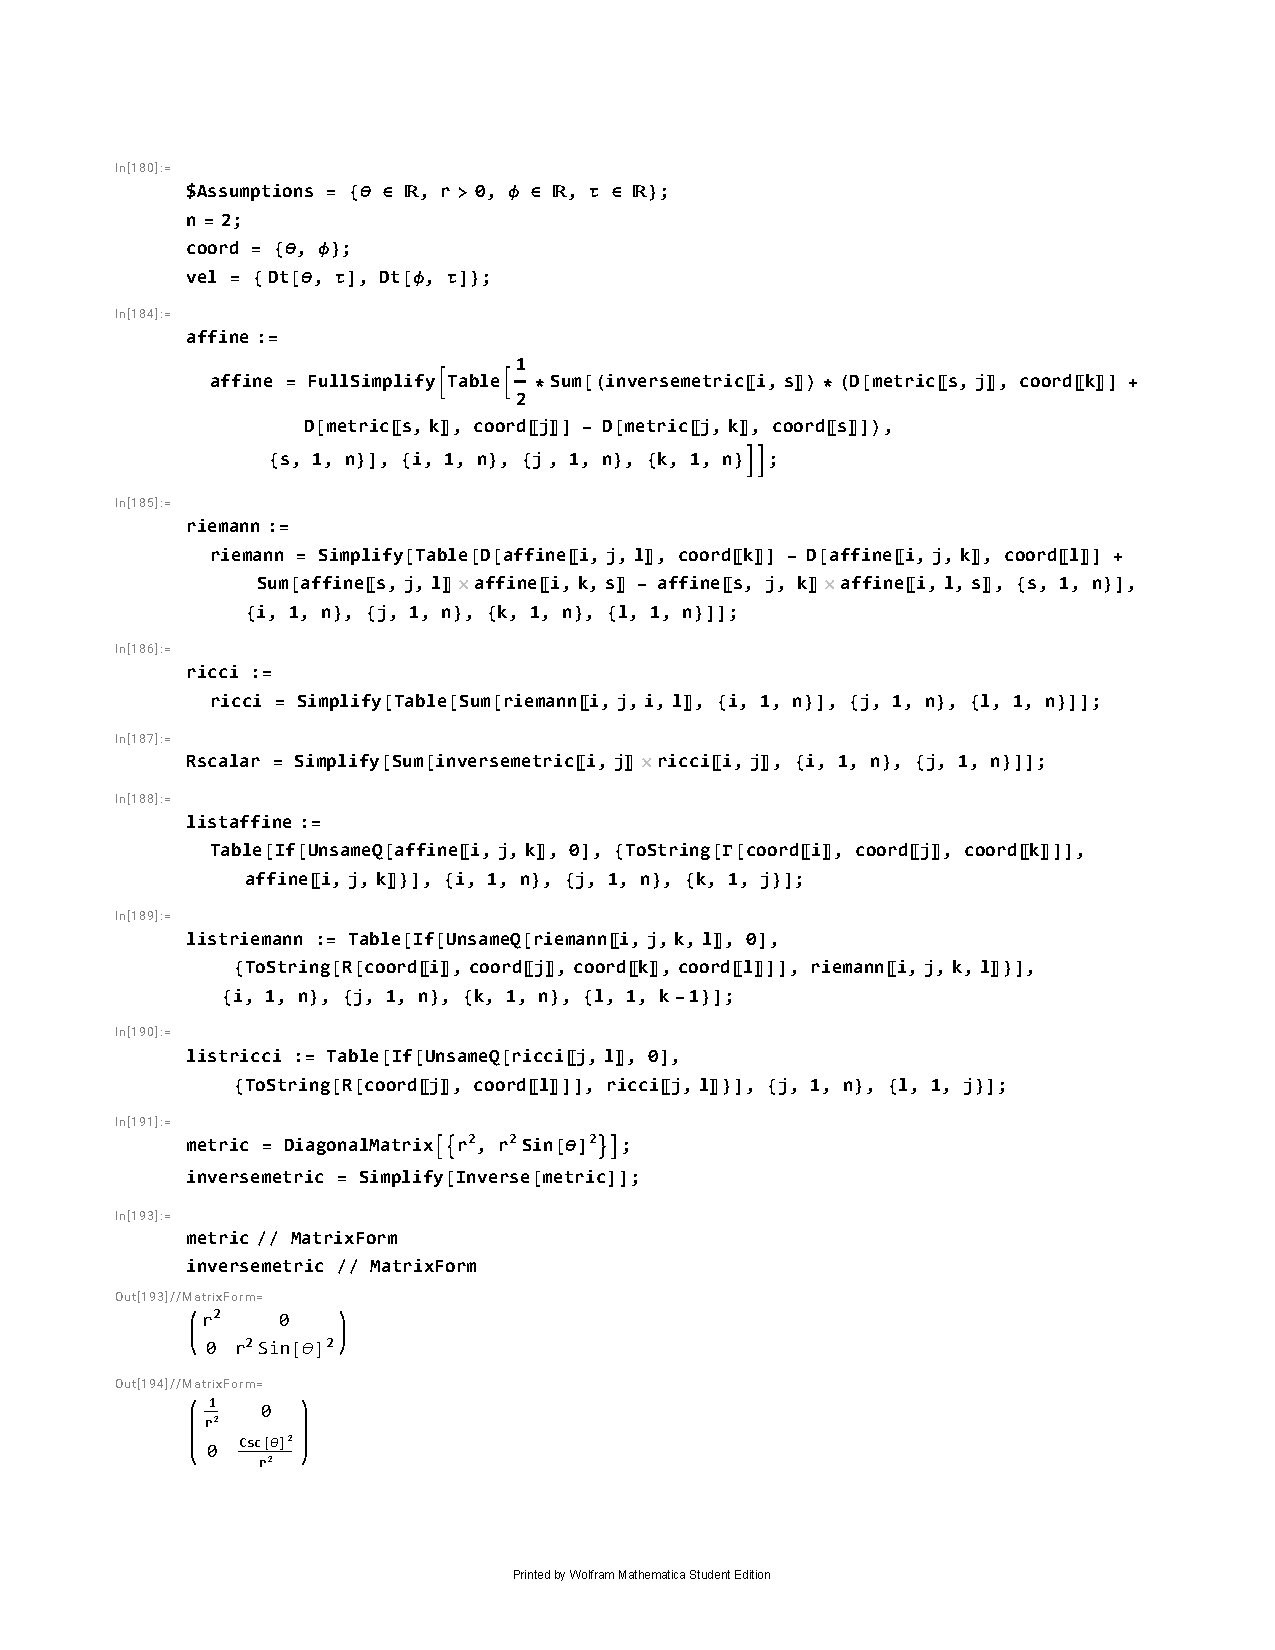
\includepdf[pages=-]{calcs/prob1.pdf}

\end{document}